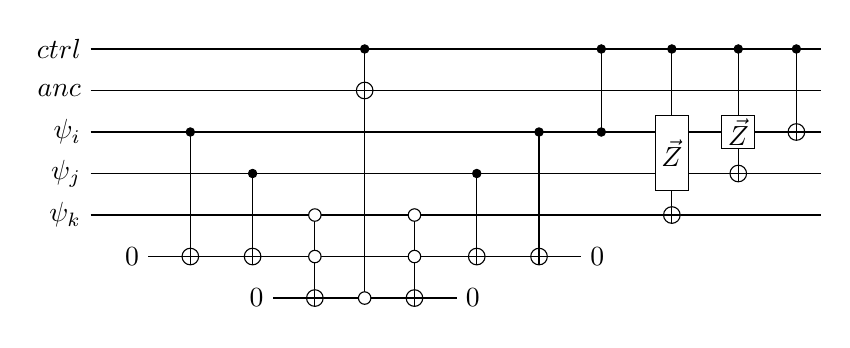
\begin{tikzpicture}[scale=1.000000,x=1pt,y=1pt]
\filldraw[color=white] (0.000000, -7.500000) rectangle (264.000000, 97.500000);
% Drawing wires
% Line 1: ctrl W ctrl
\draw[color=black] (0.000000,90.000000) -- (264.000000,90.000000);
\draw[color=black] (0.000000,90.000000) node[left] {$ctrl$};
% Line 2: anc W anc
\draw[color=black] (0.000000,75.000000) -- (264.000000,75.000000);
\draw[color=black] (0.000000,75.000000) node[left] {$anc$};
% Line 3: i W \psi_i
\draw[color=black] (0.000000,60.000000) -- (264.000000,60.000000);
\draw[color=black] (0.000000,60.000000) node[left] {$\psi_i$};
% Line 4: j W \psi_j
\draw[color=black] (0.000000,45.000000) -- (264.000000,45.000000);
\draw[color=black] (0.000000,45.000000) node[left] {$\psi_j$};
% Line 5: k W \psi_k
\draw[color=black] (0.000000,30.000000) -- (264.000000,30.000000);
\draw[color=black] (0.000000,30.000000) node[left] {$\psi_k$};
% Line 6: c0 W 0 0
\draw[color=black] (13.500000,15.000000) -- (184.500000,15.000000);
% Line 7: c1 W 0 0
\draw[color=black] (58.500000,0.000000) -- (139.500000,0.000000);
% Done with wires; drawing gates
% Line 9: c0 START
\draw[color=black] (21.000000,15.000000) node[fill=white,left,minimum height=15.000000pt,minimum width=15.000000pt,inner sep=0pt] {\phantom{$0$}};
\draw[color=black] (21.000000,15.000000) node[left] {$0$};
% Line 10: i +c0
\draw (36.000000,60.000000) -- (36.000000,15.000000);
\filldraw (36.000000, 60.000000) circle(1.500000pt);
\begin{scope}
\draw[fill=white] (36.000000, 15.000000) circle(3.000000pt);
\clip (36.000000, 15.000000) circle(3.000000pt);
\draw (33.000000, 15.000000) -- (39.000000, 15.000000);
\draw (36.000000, 12.000000) -- (36.000000, 18.000000);
\end{scope}
% Line 11: j +c0
\draw (58.500000,45.000000) -- (58.500000,15.000000);
\filldraw (58.500000, 45.000000) circle(1.500000pt);
\begin{scope}
\draw[fill=white] (58.500000, 15.000000) circle(3.000000pt);
\clip (58.500000, 15.000000) circle(3.000000pt);
\draw (55.500000, 15.000000) -- (61.500000, 15.000000);
\draw (58.500000, 12.000000) -- (58.500000, 18.000000);
\end{scope}
% Line 12: c1 START
\draw[color=black] (66.000000,0.000000) node[fill=white,left,minimum height=15.000000pt,minimum width=15.000000pt,inner sep=0pt] {\phantom{$0$}};
\draw[color=black] (66.000000,0.000000) node[left] {$0$};
% Line 13: -k -c0 +c1
\draw (81.000000,30.000000) -- (81.000000,0.000000);
\draw[fill=white] (81.000000, 30.000000) circle(2.250000pt);
\draw[fill=white] (81.000000, 15.000000) circle(2.250000pt);
\begin{scope}
\draw[fill=white] (81.000000, 0.000000) circle(3.000000pt);
\clip (81.000000, 0.000000) circle(3.000000pt);
\draw (78.000000, 0.000000) -- (84.000000, 0.000000);
\draw (81.000000, -3.000000) -- (81.000000, 3.000000);
\end{scope}
% Line 14: ctrl -c1 +anc
\draw (99.000000,90.000000) -- (99.000000,0.000000);
\filldraw (99.000000, 90.000000) circle(1.500000pt);
\draw[fill=white] (99.000000, 0.000000) circle(2.250000pt);
\begin{scope}
\draw[fill=white] (99.000000, 75.000000) circle(3.000000pt);
\clip (99.000000, 75.000000) circle(3.000000pt);
\draw (96.000000, 75.000000) -- (102.000000, 75.000000);
\draw (99.000000, 72.000000) -- (99.000000, 78.000000);
\end{scope}
% Line 15: -k -c0 +c1
\draw (117.000000,30.000000) -- (117.000000,0.000000);
\draw[fill=white] (117.000000, 30.000000) circle(2.250000pt);
\draw[fill=white] (117.000000, 15.000000) circle(2.250000pt);
\begin{scope}
\draw[fill=white] (117.000000, 0.000000) circle(3.000000pt);
\clip (117.000000, 0.000000) circle(3.000000pt);
\draw (114.000000, 0.000000) -- (120.000000, 0.000000);
\draw (117.000000, -3.000000) -- (117.000000, 3.000000);
\end{scope}
% Line 16: c1 END
\draw[color=black] (132.000000,0.000000) node[fill=white,right,minimum height=15.000000pt,minimum width=15.000000pt,inner sep=0pt] {\phantom{$0$}};
\draw[color=black] (132.000000,0.000000) node[right] {$0$};
% Line 17: j +c0
\draw (139.500000,45.000000) -- (139.500000,15.000000);
\filldraw (139.500000, 45.000000) circle(1.500000pt);
\begin{scope}
\draw[fill=white] (139.500000, 15.000000) circle(3.000000pt);
\clip (139.500000, 15.000000) circle(3.000000pt);
\draw (136.500000, 15.000000) -- (142.500000, 15.000000);
\draw (139.500000, 12.000000) -- (139.500000, 18.000000);
\end{scope}
% Line 18: i +c0
\draw (162.000000,60.000000) -- (162.000000,15.000000);
\filldraw (162.000000, 60.000000) circle(1.500000pt);
\begin{scope}
\draw[fill=white] (162.000000, 15.000000) circle(3.000000pt);
\clip (162.000000, 15.000000) circle(3.000000pt);
\draw (159.000000, 15.000000) -- (165.000000, 15.000000);
\draw (162.000000, 12.000000) -- (162.000000, 18.000000);
\end{scope}
% Line 19: c0 END
\draw[color=black] (177.000000,15.000000) node[fill=white,right,minimum height=15.000000pt,minimum width=15.000000pt,inner sep=0pt] {\phantom{$0$}};
\draw[color=black] (177.000000,15.000000) node[right] {$0$};
% Line 21: ctrl i
\draw (184.500000,90.000000) -- (184.500000,60.000000);
\filldraw (184.500000, 90.000000) circle(1.500000pt);
\filldraw (184.500000, 60.000000) circle(1.500000pt);
% Line 23: i j G $\vec{Z}$ ctrl +k
\draw (210.000000,90.000000) -- (210.000000,30.000000);
\begin{scope}
\draw[fill=white] (210.000000, 52.500000) +(-45.000000:8.485281pt and 19.091883pt) -- +(45.000000:8.485281pt and 19.091883pt) -- +(135.000000:8.485281pt and 19.091883pt) -- +(225.000000:8.485281pt and 19.091883pt) -- cycle;
\clip (210.000000, 52.500000) +(-45.000000:8.485281pt and 19.091883pt) -- +(45.000000:8.485281pt and 19.091883pt) -- +(135.000000:8.485281pt and 19.091883pt) -- +(225.000000:8.485281pt and 19.091883pt) -- cycle;
\draw (210.000000, 52.500000) node {$\vec{Z}$};
\end{scope}
\filldraw (210.000000, 90.000000) circle(1.500000pt);
\begin{scope}
\draw[fill=white] (210.000000, 30.000000) circle(3.000000pt);
\clip (210.000000, 30.000000) circle(3.000000pt);
\draw (207.000000, 30.000000) -- (213.000000, 30.000000);
\draw (210.000000, 27.000000) -- (210.000000, 33.000000);
\end{scope}
% Line 24: i G $\vec{Z}$ ctrl +j
\draw (234.000000,90.000000) -- (234.000000,45.000000);
\begin{scope}
\draw[fill=white] (234.000000, 60.000000) +(-45.000000:8.485281pt and 8.485281pt) -- +(45.000000:8.485281pt and 8.485281pt) -- +(135.000000:8.485281pt and 8.485281pt) -- +(225.000000:8.485281pt and 8.485281pt) -- cycle;
\clip (234.000000, 60.000000) +(-45.000000:8.485281pt and 8.485281pt) -- +(45.000000:8.485281pt and 8.485281pt) -- +(135.000000:8.485281pt and 8.485281pt) -- +(225.000000:8.485281pt and 8.485281pt) -- cycle;
\draw (234.000000, 60.000000) node {$\vec{Z}$};
\end{scope}
\filldraw (234.000000, 90.000000) circle(1.500000pt);
\begin{scope}
\draw[fill=white] (234.000000, 45.000000) circle(3.000000pt);
\clip (234.000000, 45.000000) circle(3.000000pt);
\draw (231.000000, 45.000000) -- (237.000000, 45.000000);
\draw (234.000000, 42.000000) -- (234.000000, 48.000000);
\end{scope}
% Line 25: ctrl +i
\draw (255.000000,90.000000) -- (255.000000,60.000000);
\filldraw (255.000000, 90.000000) circle(1.500000pt);
\begin{scope}
\draw[fill=white] (255.000000, 60.000000) circle(3.000000pt);
\clip (255.000000, 60.000000) circle(3.000000pt);
\draw (252.000000, 60.000000) -- (258.000000, 60.000000);
\draw (255.000000, 57.000000) -- (255.000000, 63.000000);
\end{scope}
% Done with gates; drawing ending labels
% Done with ending labels; drawing cut lines and comments
% Done with comments
\end{tikzpicture}
